\documentclass{wfiisul}

\usepackage[utf8]{inputenc}
\usepackage{amsmath}
\usepackage{tabularx}
\usepackage[hidelinks]{hyperref}
\usepackage{afterpage}

%\usepackage{pdflscape}
%\usepackage{afterpage}
%\usepackage{changepage}
%\usepackage{caption}
%\usepackage{rotating} %for sidewisetable
%\usepackage{makecell}
%\usepackage{boldline}
%\usepackage{amsthm}
%\usepackage{amsopn}
%\usepackage{wrapfig}
%\usepackage[table]{xcolor}

\usepackage{framed}
\usepackage{listings}
\usepackage[most]{tcolorbox}
\usepackage{hyphenat}

\hyphenation{pra-cy}

\begin{document}

\tytul{Zastosowanie ABM do analizy procesu formowania opinii w wielowymiarowej przestrzeni opinii}

\autor{Mateusz Borowiec}
\nralbumu{382765}

\promotor{Dr hab. Tomasz Gwizdałła, prof. UŁ}
\katedra{Systemów Inteligentnych}

\kierunek{informatyka}

\specjalnosc{informatyka stosowana}
\typpracy{magisterska}
\sciezka{Sztuczna inteligencja}

\stronatytulowa

%%%%%%%%%%%%%%%%%%%%%%%%%%%%%%%%%%%%%%%%%%%%%%%%%%%%%%%%%%%%%%%%%%%%%%%%%%%%%%%%%%%%%%%%%%%%%%%%%%%%%%%%%%%%%%%%%%%%%%%%%%%%%%%%%%%%%%%%%%%%%%%%%%%%%%%%%%%%%%%%%%%%%%%%%%%%%%%%%%%%%%%%%%%%%%%%%%%%%%%%%%%%%%%%%%


\chapter{Wstęp}



%%%%%%%%%%%%%%%%%%%%%%%%%%%%%%%%%%%%%%%%%%%%%%%%%%%%%%%%%%%%%%%%%%%%%%%%%%%%%%%%%%%%%%%%%%%%%%%%%%%%%%%%%%%%%%%%%%%%%%%%%%%%%%%%%%%%%%%%%%%%%%%%%%%%%%%%%%%%%%%%%%%%%%%%%%%%%%%%%%%%%%%%%%%%%%%%%%%%%%%%%%%%%%%%%%

\chapter{Podstawy teoretyczne}

\section{Czym jest ABM?}
Agent-Based Modeling (ABM) to metoda symulacji, w której jednostki zwane agentami oddziałują ze sobą oraz z otoczeniem według zdefiniowanych reguł \cite{Macal2010}.
\\ Każdy agent może mieć unikalne cechy, preferencje i zachowania, co umożliwia modelowanie różnorodności występującej w rzeczywistych systemach.
\\ Dzięki tym interakcjom można badać złożone zachowania i wzorce, które wyłaniają się na poziomie systemu.
\\ Globalne wzorce zachowań systemu wyłaniają się z interakcji między jednostkowymi agentami, co oznacza, że zachowanie całego systemu nie jest wprost zaprogramowane, ale wynika z lokalnych interakcji.
\\ Agenci mogą uczyć się i dostosowywać swoje zachowania w odpowiedzi na zmieniające się warunki otoczenia lub na podstawie doświadczeń.

ABM ma wiele zastosowań w badaniach nad systemami złożonymi w wielu dziedzinach, takich jak:

\begin{itemize}
    \item \textbf{Ekonomia i finanse:} Analiza zachowań konsumentów, rynków finansowych, decyzji inwestycyjnych oraz dynamiki makroekonomicznej \cite{Tesfatsion2006}.
    \item \textbf{Nauki społeczne:} Modelowanie procesów społecznych, takich jak dyfuzja innowacji, zachowania tłumu, ewolucja norm społecznych oraz migracje \cite{Epstein2007}.
    \item \textbf{Biologia i ekologia:} Badanie dynamiki populacji, interakcji międzygatunkowych, rozprzestrzeniania się chorób oraz zachowań zwierząt \cite{Grimm2005}.
    \item \textbf{Inżynieria i urbanistyka:} Symulacje ruchu drogowego, optymalizacja planowania urbanistycznego, zarządzanie infrastrukturą i systemami transportowymi \cite{Bonabeau2002}.
    \item \textbf{Epidemiologia:} Modelowanie rozprzestrzeniania się chorób zakaźnych, skuteczności interwencji zdrowotnych, oraz dynamiki szczepień \cite{Eubank2004}.
\end{itemize}

\section{Sieci społecznościowe}
Sieci społecznościowe to struktury złożone z jednostek (węzłów) oraz powiązań między nimi (krawędzi), które modelują relacje społeczne lub interakcje pomiędzy różnymi podmiotami.
\\ Jednostkami w takich sieciach mogą być osoby, organizacje, grupy społeczne lub inne podmioty,
a relacje między nimi mogą obejmować przyjaźnie, współpracę, przepływ informacji, wpływy lub inne formy interakcji społecznych.

\subsection{Elementy sieci społecznościowych}
Sieci społecznościowe można opisywać i analizować za pomocą teorii grafów, gdzie węzły odpowiadają aktorom społecznym, a krawędzie – relacjom między nimi \cite{Wasserman1994}.
\\ W teorii grafów sieć społeczna jest grafem, który może być skierowany lub nieskierowany, w zależności od tego, czy relacje między węzłami są wzajemne, oraz ważony, gdy krawędzie mają przypisane wartości liczbowe,
odzwierciedlające np. siłę lub intensywność relacji między węzłami. Na przykład, w sieci znajomości wagi mogą odzwierciedlać częstotliwość interakcji.
\\ Sieci często wykazują pewne struktury, w których węzły są bardziej gęsto połączone ze sobą niż z innymi częściami sieci, tworząc tzw. społeczności \cite{Girvan2002}.
\\ Niektóre węzły w sieci mogą odgrywać również bardziej centralną rolę, np. poprzez łączenie wielu innych węzłów lub pośrednictwo w przepływie informacji \cite{Freeman1979}.

\subsection{Rodzaje sieci społecznościowych}
\begin{itemize}
      \item \textbf{Sieci egocentryczne:} Sieci, które koncentrują się na pojedynczym węźle (osobie lub organizacji) oraz jego bezpośrednich połączeniach.
            \\ Analiza takiej sieci pokazuje, jak jednostka jest powiązana z innymi aktorami \cite{Hanneman2005}.
      \item \textbf{Sieci pełne:} Sieci, które obejmują całą grupę lub populację i badają relacje pomiędzy wszystkimi jednostkami w tej grupie.
            \\ Są one szczególnie użyteczne do analizy struktur globalnych, takich jak hierarchie czy przepływy informacji \cite{Scott2000}.
      \item \textbf{Sieci jednopoziomowe:} W tego rodzaju sieciach każdy węzeł reprezentuje ten sam typ jednostek, np. osoby lub organizacje,
            a krawędzie to relacje między nimi \cite{Newman2010}.
      \item \textbf{Sieci dwupoziomowe:} Sieci te zawierają dwa typy węzłów, np. osoby i wydarzenia, a krawędzie reprezentują uczestnictwo danej osoby w wydarzeniu \cite{Borgatti1997}.
      \item \textbf{Sieci dynamiczne:} Sieci, w których relacje między węzłami mogą zmieniać się w czasie.
            \\ Tego typu sieci są szczególnie przydatne w badaniu ewolucji grup społecznych, migracji czy zmian w przepływie informacji \cite{Holme2012}.
\end{itemize}

W pracy przeanalizowane zostaną najważniejsze modele losowych grafów: model Erdős-Rényi, model Barabási-Albert, oraz model Watts–Strogatz.
\section{Sieć Erdős-Rényi}
Model sieci Erdős-Rényi (ER) jest jednym z najprostszych i najwcześniejszych modeli matematycznych do generowania losowych sieci.
Nazwa pochodzi od nazwisk dwóch matematyków, Paula Erdősa i Alfréda Rényi, którzy w 1959 roku zaproponowali ten model \cite{Erdos1959}.
Model ten jest często stosowany jako punkt odniesienia w analizie sieci i badaniach naukowych dotyczących struktur sieciowych.

\subsection{Definicja modelu Erdős-Rényi}
Istnieją dwie podstawowe wersje modelu Erdős-Rényi:

\begin{itemize}
      \item \textbf{Model $G(n, M)$}: Dany jest zbiór $n$ węzłów, a następnie losowo wybierane jest dokładnie $M$ krawędzi spośród wszystkich możliwych par węzłów.
            Każda z $M$ krawędzi jest dodawana niezależnie.
      \item \textbf{Model $G(n, p)$}: Dany jest zbiór $n$ węzłów, a każda para węzłów jest połączona krawędzią z prawdopodobieństwem $p$, niezależnie od innych par.
            Ostateczna liczba krawędzi w tej wersji jest zmienną losową.
\end{itemize}

Najczęściej stosowaną wersją jest model $G(n, p)$, który jest bardziej intuicyjny i daje większą elastyczność w kontroli gęstości sieci.

\subsection{Właściwości sieci Erdős-Rényi}
\begin{itemize}
      \item \textbf{Rozkład stopni węzłów:} W modelu $G(n, p)$ stopień każdego węzła jest zmienną losową o rozkładzie dwumianowym $Bin(n - 1, p)$.
            Dla dużych $n$ rozkład ten zbliża się do rozkładu Poissona o wartości oczekiwanej $\lambda = p(n - 1)$.
      \item \textbf{Średnia długość najkrótszej ścieżki:} W miarę wzrostu liczby węzłów $n$, średnia odległość między węzłami jest stosunkowo krótka, rzędu $\ln n / \ln (np)$,
            co jest typowe dla tzw. efektu „małego świata”.
      \item \textbf{Klasteryzacja:} W sieci Erdős-Rényi współczynnik klasteryzacji, czyli prawdopodobieństwo, że dwa węzły sąsiadujące z danym węzłem są również połączone ze sobą,
            jest rzędu $p$ i nie zależy od lokalnych struktur.
      \item \textbf{Pojawienie się gigantycznego składnika:} W modelu $G(n, p)$ istnieje próg $p_c = \frac{1}{n}$,
            powyżej którego zaczyna się tworzyć tzw. gigantyczny składnik – duża, spójna część sieci obejmująca znaczną część węzłów.
      \item \textbf{Losowy charakter:} Sieć nie posiada regularnej struktury, a rozmieszczenie krawędzi jest całkowicie losowe.
\end{itemize}

\subsection{Zastosowania sieci Erdős-Rényi}
Model Erdős-Rényi stanowi podstawę teoretyczną do badań nad sieciami losowymi i służy jako punkt odniesienia w analizie bardziej złożonych struktur sieciowych.
Choć rzadko spotyka się go w rzeczywistych sieciach (np. sieciach społecznościowych, biologicznych, komputerowych), pomaga on zrozumieć, jak różnią się rzeczywiste sieci od struktur losowych.

\subsection{Ograniczenia modelu Erdős-Rényi}
Model Erdős-Rényi nie odzwierciedla dobrze wielu cech rzeczywistych sieci:
\begin{itemize}
      \item \textbf{Mała klasteryzacja:} Rzeczywiste sieci często mają znacznie wyższy współczynnik klasteryzacji niż sieć ER.
      \item \textbf{Rozkład stopni węzłów:} W sieci ER stopnie węzłów mają rozkład zbliżony do Poissona,
            podczas gdy wiele rzeczywistych sieci charakteryzuje się rozkładem potęgowym (np. większość węzłów ma niski stopień, ale istnieje kilka węzłów o bardzo wysokim stopniu).
\end{itemize}
\section{Sieć Barabási-Albert}
Model Barabási-Albert (BA) to model sieci bezskalowej, gdzie stopnie węzłów podążają za rozkładem potęgowym.
Model ten został zaproponowany przez Alberta-László Barabásiego i Rékę Alberta w 1999 roku \cite{Barabasi1999} i jest jednym z najważniejszych modeli do opisu sieci rzeczywistych,
takich jak sieci społecznościowe, internet, sieci metaboliczne i wiele innych.

\subsection{Założenia modelu Barabási-Albert}
Model BA opiera się na dwóch kluczowych mechanizmach:

\begin{itemize}
      \item \textbf{Preferencyjne przyłączanie:} Nowe węzły mają większe prawdopodobieństwo połączenia się z węzłami, które już mają wiele połączeń.
            \\ Oznacza to, że „bogaci stają się bogatsi” - węzły o wysokim stopniu przyciągają więcej nowych połączeń.
      \item \textbf{Wzrost:} Sieć rozwija się w czasie, przy czym do istniejącej sieci dodawane są nowe węzły, które tworzą połączenia z już istniejącymi węzłami.
\end{itemize}

\subsection{Algorytm generowania sieci Barabási-Albert}
Proces budowania sieci BA jest następujący:

\begin{enumerate}
      \item \textbf{Inicjalizacja:} Rozpocznij od małej sieci początkowej składającej się z $m_0$ węzłów, które są połączone w pewien sposób.
      \item \textbf{Dodawanie nowego węzła:} Na każdym kroku dodawany jest nowy węzeł, który tworzy $m \leq m_0$ krawędzi łączących go z już istniejącymi węzłami.
      \item \textbf{Preferencyjne przyłączanie:} Prawdopodobieństwo, że nowy węzeł połączy się z istniejącym węzłem $i$, jest proporcjonalne do stopnia węzła $k_i$. Formalnie, prawdopodobieństwo to wynosi:
            \begin{equation}
                  \Pi(k_i) = \frac{k_i}{\sum_{j} k_j}
                  \label{eq:preferential-attachment-probability}
            \end{equation}
            gdzie $k_i$ to stopień węzła $i$, a suma w mianowniku przebiega przez wszystkie istniejące węzły w sieci.
\end{enumerate}

Proces ten jest kontynuowany, aż sieć osiągnie oczekiwaną liczbę węzłów.

\subsection{Właściwości sieci Barabási-Albert}
Model Barabási-Albert opisuje sposób, w jaki sieci rozwijają się zgodnie z zasadą preferencyjnego przyłączania. Model ten ma pewne charakterystyczne właściwości:

\begin{itemize}
      \item \textbf{Preferencyjne przyłączanie:} Nowo dodawane węzły mają większe prawdopodobieństwo połączenia się z węzłami, które już mają dużą liczbę połączeń.
            Oznacza to, że węzły z większą liczbą połączeń (tzw. huby) rosną szybciej, co prowadzi do tworzenia się kilku bardzo dobrze połączonych węzłów w sieci \cite{Barabasi1999}.

      \item \textbf{Rozkład potęgowy stopni węzłów:} Stopnie węzłów w sieci BA (liczba połączeń węzła) podążają za rozkładem potęgowym.
            \\ Oznacza to, że większość węzłów ma niewiele połączeń, ale istnieje niewielka liczba węzłów o bardzo dużej liczbie połączeń.
            Rozkład ten charakteryzuje się rzadkim występowaniem węzłów o bardzo wysokim stopniu, co opisuje wzór:
            \begin{equation}
                  P(k) \sim k^{-\gamma}
                  \label{eq:power-law-probability}
            \end{equation}
            gdzie $P(k)$ jest prawdopodobieństwem, że węzeł ma $k$ połączeń, a $\gamma$ jest parametrem rozkładu, zwykle w przybliżeniu równym 3 \cite{Barabasi1999}.

      \item \textbf{Skalowalność:} Sieci BA są \textit{skalowalne}, co oznacza, że właściwości topologiczne sieci nie zależą od jej wielkości.
            Wzorce łączenia się węzłów pozostają podobne niezależnie od liczby węzłów w sieci, a sieć rozwija się zgodnie z tymi samymi regułami, niezależnie od jej rozmiaru \cite{Newman2003}.

      \item \textbf{Bezskalowość:} Sieci BA są sieciami \textit{bezskalowymi}, co oznacza, że nie ma typowego rozmiaru węzła (stopnia węzła).
            Dominują węzły o małej liczbie połączeń, ale możliwe jest istnienie węzłów o bardzo wysokim stopniu, co różni je od sieci losowych z rozkładem Poissona \cite{Albert2002}.

      \item \textbf{Odporność na uszkodzenia losowe:} Sieci o strukturze BA są stosunkowo odporne na losowe usunięcie węzłów.
            Nawet po usunięciu dużej liczby losowo wybranych węzłów, sieć może nadal funkcjonować, ponieważ większość węzłów ma niewielką liczbę połączeń.
            Jednak sieć jest podatna na ukierunkowane ataki na huby, ponieważ ich usunięcie może prowadzić do fragmentacji sieci \cite{Albert2000}.
\end{itemize}

\subsection{Zastosowania sieci Barabási-Albert}
Model BA dobrze opisuje strukturę wielu rzeczywistych sieci, w tym:
\begin{itemize}
      \item \textbf{Sieci internetowe:} Węzły reprezentują strony internetowe, a krawędzie — linki między nimi. Występuje kilka stron (hubów) mających bardzo dużą liczbę połączeń.
      \item \textbf{Sieci społecznościowe:} Węzły reprezentują osoby, a krawędzie ich relacje społeczne. Niektóre osoby (np. celebryci) mają znacznie więcej połączeń niż inne.
      \item \textbf{Sieci biologiczne:} W sieciach metabolicznych czy sieciach interakcji białek obserwuje się strukturę skali bez charakterystycznej wielkości.

      \item \textbf{Internet i sieci komputerowe:} Internet można modelować jako sieć BA, gdzie węzły reprezentują routery lub serwery, a krawędzie – połączenia między nimi.
            Zasada preferencyjnego przyłączania dobrze odzwierciedla sposób, w jaki nowe witryny internetowe łączą się z popularnymi stronami, tworząc kilka hubów,
            które odpowiadają głównym węzłom sieciowym \cite{Barabasi2003}.

      \item \textbf{Biologia i sieci metaboliczne:} Sieci BA mają zastosowanie w biologii, zwłaszcza w analizie sieci metabolicznych organizmów, gdzie metabolity (węzły) są połączone reakcjami enzymatycznymi (krawędzie).
            Takie sieci również wykazują rozkład potęgowy, z kilkoma metabolitami o bardzo dużej liczbie połączeń, co sprawia, że sieci metaboliczne są odporne na przypadkowe zakłócenia \cite{Jeong2000}.

      \item \textbf{Ekonomia i finanse:} Model BA jest używany do opisu systemów ekonomicznych, takich jak sieci handlowe, gdzie firmy, instytucje finansowe lub rynki są węzłami, a ich wzajemne relacje, jak np. kontrakty, to krawędzie.
            \\ W tych systemach preferencyjne przyłączanie odzwierciedla, jak większe firmy przyciągają więcej partnerów biznesowych, tworząc sieci z rozkładem potęgowym \cite{Battiston2007}.

      \item \textbf{Nauka i sieci cytowań:} W badaniach naukowych model BA jest wykorzystywany do opisu sieci cytowań, gdzie węzłami są artykuły naukowe, a krawędzie oznaczają cytowania między nimi.
            Starsze, bardziej cytowane artykuły są częściej cytowane przez nowe prace, co tworzy strukturę sieci z kilkoma bardzo często cytowanymi artykułami w roli hubów \cite{Price1976}.

      \item \textbf{Media społecznościowe:} Sieci BA są również stosowane w analizie sieci społecznościowych, takich jak Facebook, Twitter czy LinkedIn.
            Użytkownicy tych platform (węzły) tworzą połączenia (krawędzie) z innymi użytkownikami, a zasada preferencyjnego przyłączania powoduje, że popularni użytkownicy (huby) zdobywają jeszcze więcej połączeń,
            co prowadzi do powstawania struktur bezskalowych \cite{Leskovec2008}.
            \newpage

      \item \textbf{Propagacja informacji i epidemie:} Sieci BA znajdują zastosowanie w modelowaniu rozprzestrzeniania się informacji lub chorób w sieciach społecznych.
            Model BA może symulować, jak epidemie lub plotki szybko rozprzestrzeniają się przez kilka kluczowych węzłów (osób o wysokiej liczbie połączeń),
            co pomaga w opracowywaniu strategii kontroli lub przewidywania rozwoju epidemii \cite{Pastor2001}.
\end{itemize}

\subsection{Ograniczenia modelu Barabási-Albert}
Mimo że model BA jest użyteczny, ma pewne ograniczenia:

\begin{itemize}
      \item \textbf{Zbyt uproszczona struktura sieci:} Model BA zakłada, że nowe węzły łączą się tylko na podstawie preferencyjnego przyłączania,
            gdzie prawdopodobieństwo połączenia się z istniejącym węzłem zależy od liczby jego połączeń.
            \\ W rzeczywistych sieciach istnieje jednak wiele innych czynników wpływających na tworzenie połączeń, takich jak geografia, interesy, zasoby, które model BA ignoruje \cite{Newman2003}.

      \item \textbf{Brak heterogeniczności w węzłach:} W modelu BA wszystkie węzły są traktowane jako jednorodne i mają te same właściwości poza liczbą połączeń.
            W rzeczywistości węzły różnią się wieloma cechami, takimi jak zdolności przetwarzania informacji, rola w sieci, czy preferencje, co może wpływać na sposób, w jaki tworzą połączenia \cite{Klemm2002}.

      \item \textbf{Brak uwzględnienia ograniczeń topologicznych:} W modelu BA nie ma ograniczeń dotyczących liczby połączeń, które może mieć węzeł.
            \\ W rzeczywistych sieciach, takich jak sieci społeczne czy biologiczne, istnieją fizyczne lub społeczne ograniczenia na liczbę relacji, które jeden węzeł może utrzymywać, co model BA pomija \cite{Amaral2000}.

      \item \textbf{Zbyt prosty mechanizm wzrostu:} Sieci rzeczywiste rozwijają się często w sposób bardziej złożony, niż sugeruje to model BA.
            Wiele sieci rozwija się nie tylko poprzez przyłączanie nowych węzłów do istniejących, ale także poprzez usuwanie węzłów, zmiany w strukturze połączeń,
            czy tworzenie nowych krawędzi między istniejącymi węzłami, czego model BA nie uwzględnia \cite{Dorogovtsev2002}.

      \item \textbf{Nierealność preferencyjnego przyłączania w pewnych kontekstach:} Zasada preferencyjnego przyłączania, na której opiera się model BA,
            zakłada, że węzły z większą liczbą połączeń zawsze przyciągają więcej nowych połączeń.
            W wielu przypadkach, np. w sieciach społecznych lub ekonomicznych, inne czynniki,
            takie jak reputacja, dostępność lub jakość zasobów, mogą odgrywać większą rolę niż sama liczba połączeń \cite{Boccaletti2006}.

      \item \textbf{Brak dynamiki krawędzi:} W modelu BA nowe węzły dodają nowe krawędzie, ale nie ma możliwości modyfikowania istniejących połączeń ani usuwania starych.
            W rzeczywistych sieciach krawędzie mogą zanikać, np. w wyniku przestarzałych kontaktów, zmian w interesach lub rozwoju technologii \cite{Holme2002}.
\end{itemize}

\section{Sieć Watts-Strogatz}
Model sieci Watts-Strogatz (WS) jest jednym z kluczowych modeli do analizy zjawiska tzw. małego świata w sieciach.
Został zaproponowany przez Duncana Wattsa i Stevena Strogatza w 1998 roku \cite{Watts1998}.
Model ten pozwala generować sieci, które łączą w sobie cechy zarówno sieci regularnych, jak i losowych, co czyni go użytecznym w opisie rzeczywistych sieci społecznych, biologicznych czy technologicznych.

\subsection{Cechy modelu Watts-Strogatz}
Sieci Watts-Strogatz charakteryzują się następującymi właściwościami:
\begin{itemize}
    \item \textbf{Krótka średnia ścieżka:} Węzły są od siebie oddzielone przez stosunkowo małą liczbę połączeń, co jest charakterystyczne dla sieci „małego świata” \cite{Watts1998}.
    \item \textbf{Wysoki współczynnik klasteryzacji:} Węzły są silnie połączone z sąsiadami, tworząc lokalne grupy (kliki), co odpowiada klasteryzacji obserwowanej w rzeczywistych sieciach \cite{Watts1998}.
    \item \textbf{Efekt małego świata:} Sieć Watts-Strogatz stanowi pośrednią strukturę pomiędzy sieciami regularnymi (gdzie węzły są połączone według ustalonego wzorca) a sieciami losowymi (gdzie połączenia są tworzone przypadkowo) \cite{Watts1998}.
\end{itemize}

\subsection{Algorytm generowania sieci Watts-Strogatz}
Proces generowania sieci WS przebiega następująco:

\begin{enumerate}
    \item \textbf{Konstrukcja pierścienia:} Rozpocznij od utworzenia regularnego pierścienia z $n$ węzłami,
          gdzie każdy węzeł jest połączony z $k/2$ najbliższymi sąsiadami z każdej strony (czyli każdy węzeł ma $k$ połączeń).
    \item \textbf{Przełączanie krawędzi:} Dla każdej krawędzi łączącej węzeł $i$ z węzłem $j$, losowo przełącz ją z prawdopodobieństwem $p$ na nową krawędź,
          łącząc $i$ z losowo wybranym węzłem $m$, pod warunkiem, że nie ma już połączenia między $i$ a $m$.
\end{enumerate}

Parametr $p$ kontroluje stopień losowości w sieci:
\begin{itemize}
    \item Dla $p = 0$ sieć jest całkowicie regularna.
    \item Dla $p = 1$ sieć staje się zupełnie losowa.
    \item Dla wartości $0 < p < 1$ sieć zachowuje zarówno wysoką klasteryzację, jak i krótką średnią ścieżkę, co odpowiada strukturze „małego świata”.
\end{itemize}

\subsection{Właściwości sieci Watts-Strogatz}
Sieci Watts-Strogatz charakteryzują się następującymi właściwościami:
\begin{itemize}
    \item \textbf{Krótka średnia ścieżka:} Węzły są od siebie oddzielone przez stosunkowo małą liczbę połączeń,
          co jest charakterystyczne dla sieci „małego świata” \cite{Watts1998}.
    \item \textbf{Wysoki współczynnik klasteryzacji:} Węzły są silnie połączone z sąsiadami, tworząc lokalne grupy (kliki),
          co odpowiada klasteryzacji obserwowanej w rzeczywistych sieciach \cite{Watts1998}.
    \item \textbf{Efekt małego świata:} Sieć Watts-Strogatz stanowi pośrednią strukturę pomiędzy sieciami regularnymi (gdzie węzły są połączone według ustalonego wzorca) a sieciami losowymi (gdzie połączenia są tworzone przypadkowo) \cite{Watts1998}.
\end{itemize}

\subsection{Zastosowania sieci Watts-Strogatz}
Model Watts-Strogatz jest wykorzystywany do analizy i modelowania struktur sieciowych w różnych dziedzinach, takich jak:
\begin{itemize}
    \item \textbf{Sieci społecznościowe:} W sieciach społecznościowych znajomi często tworzą małe, silnie powiązane grupy, ale istnieją także połączenia z osobami spoza tych grup \cite{Watts1998}.
    \item \textbf{Sieci biologiczne:} Występuje w neuronowych sieciach mózgowych, gdzie niektóre neurony są bardziej skłonne do połączeń w lokalnych regionach, ale mają także połączenia do odległych obszarów \cite{Sporns2004}.
    \item \textbf{Sieci komunikacyjne i transportowe:} Takie jak sieci elektryczne czy sieci lotnicze, które mają zarówno krótkie lokalne, jak i długodystansowe połączenia \cite{Barrat2004}.
\end{itemize}

\subsection{Ograniczenia modelu Watts-Strogatz}
Chociaż model Watts-Strogatz odzwierciedla wiele cech rzeczywistych sieci, ma też pewne ograniczenia:
\begin{itemize}
    \item \textbf{Rozkład stopni węzłów:} Sieć Watts-Strogatz nie tworzy rozkładu potęgowego stopni węzłów, co ogranicza jej zdolność do odzwierciedlania struktur sieci o charakterze bezskalowym \cite{Barabasi1999}.
    \item \textbf{Brak różnorodności w ewolucji sieci:} Model nie uwzględnia mechanizmu preferencyjnego przyłączania, który jest kluczowy w wielu rzeczywistych sieciach \cite{Newman2003}.
\end{itemize}

\section{Diagram Nolana}
Diagram Nolana jest narzędziem używanym do wizualizacji spektrum politycznego, które rozszerza tradycyjny, jednowymiarowy podział na lewicę i prawicę, wprowadzając dwuwymiarową analizę poglądów politycznych.
Stworzony został przez amerykańskiego libertarianina Davida Nolana w 1970 roku \cite{Nolan1971}.
\\ Diagram ten zyskał popularność wśród osób poszukujących bardziej złożonego sposobu zrozumienia różnorodności ideologicznej, ponieważ uwzględnia zarówno kwestie ekonomiczne, jak i społeczne w analizie politycznej.

\subsection{Kontekst historyczno-naukowy}
Tradycyjne postrzeganie spektrum politycznego jako linii prostej — od skrajnej lewicy do skrajnej prawicy — zostało poddane krytyce przez badaczy, filozofów i działaczy politycznych,
którzy zauważyli, że jednowymiarowy model jest niewystarczający do opisu złożoności ideologii politycznych.
W latach 60. i 70. XX wieku pojawiło się zainteresowanie wielowymiarowym podejściem do analizy politycznej, co skłoniło Davida Nolana do opracowania bardziej złożonego modelu \cite{Nolan1971}.

Nolan zauważył, że różne ideologie mają różne podejścia do kwestii wolności osobistej oraz wolności ekonomicznej.
Jego dwuwymiarowy model pozwalał na bardziej precyzyjną identyfikację pozycji ideologicznych, zwłaszcza dla ideologii, które nie pasowały do tradycyjnej skali lewica-prawica, takich jak libertarianizm.

\subsection{Opis diagramu Nolana}
Diagram Nolana przedstawia spektrum polityczne jako kwadrat podzielony na cztery ćwiartki, które reprezentują różne orientacje polityczne:

\begin{itemize}
      \item \textbf{Oś pozioma (wolność ekonomiczna):} Reprezentuje zakres kontroli państwa nad gospodarką.
            Na lewym końcu znajdują się poglądy opowiadające się za większym wpływem rządu na kwestie ekonomiczne (np. socjalizm),
            natomiast na prawym końcu są poglądy popierające wolny rynek i minimalną interwencję rządową (np. leseferyzm).
      \item \textbf{Oś pionowa (wolność osobista):} Przedstawia zakres swobód obywatelskich i społecznych.
            Na górnym końcu znajdują się ideologie popierające maksymalną wolność osobistą (np. libertarianizm),
            podczas gdy na dolnym końcu znajdują się ideologie popierające większą kontrolę rządową nad życiem osobistym (np. autorytaryzm).
\end{itemize}

Pogranicze tych dwóch osi tworzy cztery główne obszary ideologiczne:
\begin{itemize}
      \item \textbf{Libertarianizm (prawy górny róg):} Wysoka wolność osobista i ekonomiczna.
      \item \textbf{Autorytaryzm (lewy dolny róg):} Niska wolność osobista i ekonomiczna.
      \item \textbf{Lewica (lewy górny róg):} Wysoka wolność osobista, ale niska wolność ekonomiczna.
      \item \textbf{Prawica (prawy dolny róg):} Wysoka wolność ekonomiczna, ale niska wolność osobista.
\end{itemize}

\subsection{Zastosowanie i znaczenie diagramu Nolana}
Diagram Nolana jest używany do analizy i klasyfikacji poglądów politycznych w sposób, który uwzględnia wielowymiarową naturę ideologii. Pomaga on:

\begin{itemize}
      \item \textbf{Rozszerzyć tradycyjne spektrum polityczne:} Pokazuje, że wiele ideologii nie pasuje do jednowymiarowego podziału na lewicę i prawicę,
            zwracając uwagę na to, że kwestie wolności osobistej i ekonomicznej mogą być od siebie niezależne.
      \item \textbf{Identyfikować złożone poglądy polityczne:} Umożliwia dokładniejszą \\ identyfikację pozycji ideologicznych dla jednostek lub organizacji,
            których poglądy są bardziej złożone, niż proste podziały na lewicę i prawicę.
      \item \textbf{Wspierać edukację polityczną:} Jest używany jako narzędzie dydaktyczne do nauczania o różnorodności politycznej, pomagając zrozumieć,
            jak różne ideologie odnoszą się do wolności osobistej i ekonomicznej.
\end{itemize}

\subsection{Krytyka diagramu Nolana}
Mimo swojej popularności i użyteczności, diagram Nolana jest także przedmiotem krytyki:
\begin{itemize}
      \item \textbf{Nadmierne uproszczenie:} Niektórzy badacze argumentują, że nawet model dwuwymiarowy nie oddaje pełni złożoności poglądów politycznych,
            które mogą obejmować wiele innych wymiarów, takich jak ekologia, polityka zagraniczna czy kwestie kulturowe \cite{Rothbard1978}.
      \item \textbf{Subiektywny wybór osi:} Oś wolności ekonomicznej i osobistej może nie być najważniejszym aspektem dla wszystkich osób, co sprawia, że model ten może nie być uniwersalny \cite{Kirsch2020}.
\end{itemize}


%%%%%%%%%%%%%%%%%%%%%%%%%%%%%%%%%%%%%%%%%%%%%%%%%%%%%%%%%%%%%%%%%%%%%%%%%%%%%%%%%%%%%%%%%%%%%%%%%%%%%%%%%%%%%%%%%%%%%%%%%%%%%%%%%%%%%%%%%%%%%%%%%%%%%%%%%%%%%%%%%%%%%%%%%%%%%%%%%%%%%%%%%%%%%%%%%%%%%%%%%%%%%%%%%%

\chapter{Opis metod (algorytmy, założenia, warunki graniczne)}

Agent posiada następujące parametry:

\begin{table}[htbp]
  \centering
  \begin{tabular}{c|c|c}
    \hline
    Zmienna                & Zakres wartości & Rozkład     \\
    \hline
    Wpływ na innych        & 0-1             & równomierny \\
    Elastyczność jednostki & 0,1-1           & beta        \\
    Opinia początkowa      & 0-1             & równomierny \\
  \end{tabular}
  \caption{Parametry agenta}
  \label{tab:agent_parameters}
\end{table}

Aktualizacja opinii składa się z następujących zmiennych:

\begin{table}[htbp]
  \centering
  \begin{tabular}{c|c}
    \hline
    Zmienna                                      & Zakres wartości     \\
    \hline
    Średnia opinii sąsiadów                      & 0-1                 \\
    Srednia wpływu sąsiadów                      & 0-1                 \\
    Udział znajomych agenta w populacji          & 0-1                 \\
    Odległość opinii agenta i średniej znajomych & 0-1                 \\
    Modyfikator środka rozkładu                  & Elastyczność agenta \\% * (udział znajomych agenta w populacji + wpływ sąsiadów) = [0-1] * ([0-1] + [0-1]) \\
  \end{tabular}
  \caption{Parametry aktualizacji opinii}
  \label{tab:opinion_update_parameters}
\end{table}

\section{Rozkład trójkątny}

Opinia sąsiadów:
\begin{itemize}
  \item średnia opinii sąsiadów: 0-1
  \item średnia wpływu sąsiadów: 0-1
\end{itemize}

Centrum rozkładu trójkątnego: (stopień jednostki + średnia wpływu sąsiadów) * elastyczność jednostki

Minimum rozkładu: opinia jednostki

Maksimum rozkładu: średnia opinii sąsiadów

Odległość między opiniami = abs (opinia jednostki — średnia opinii sąsiadów)

\section{Nowy modyfikator środka rozkładu}

Elastyczność agenta * średnia ([udział znajomości agenta w populacji, wpływ sąsiadów]) = [0-1] * ([0-1] * [0-1] / 2) = [0-1] * [0-1] = [0-1].

Średnia wpływu sąsiadów będzie średnią ważoną.

%%%%%%%%%%%%%%%%%%%%%%%%%%%%%%%%%%%%%%%%%%%%%%%%%%%%%%%%%%%%%%%%%%%%%%%%%%%%%%%%%%%%%%%%%%%%%%%%%%%%%%%%%%%%%%%%%%%%%%%%%%%%%%%%%%%%%%%%%%%%%%%%%%%%%%%%%%%%%%%%%%%%%%%%%%%%%%%%%%%%%%%%%%%%%%%%%%%%%%%%%%%%%%%%%%

\chapter{Opis technologii wykorzystanych w pracy}

W pracy został wykorzystany język Python do implementacji zarówno sieci społecznych, zapisu wyników, jak i wykresów obrazujących wyniki.
Główną biblioteką wykorzystywaną do implementacji sieci społecznych jest biblioteka NetworkX.
Biblioteką do tworzenia wykresów została biblioteka Matplotlib.
Do odczytu / zapisu plików CSV została użyta biblioteka `csv`.

%%%%%%%%%%%%%%%%%%%%%%%%%%%%%%%%%%%%%%%%%%%%%%%%%%%%%%%%%%%%%%%%%%%%%%%%%%%%%%%%%%%%%%%%%%%%%%%%%%%%%%%%%%%%%%%%%%%%%%%%%%%%%%%%%%%%%%%%%%%%%%%%%%%%%%%%%%%%%%%%%%%%%%%%%%%%%%%%%%%%%%%%%%%%%%%%%%%%%%%%%%%%%%%%%%

\chapter{Opis implementacji}

\section{Klasa Network}

Każda sieć społeczna składa się z grafu NetworkX oraz listy agentów, przypisanych do każdego wierzchołka.
Typ aktualizacji opinii jest również zdefiniowany w klasie.
Ponadto, do celów logowania, klasa zawiera nazwę sieci społecznej.

\section{Klasa Agent}

Każdy agent ma następujące parametry:
\begin{itemize}
  \item Wpływ na innych (influence) - Ten parametr osiąga wartości 0-1 i określa wartość wpływu na innych agentów
  \item Elastyczność (flexibility) - Osiąga wartości 0-1 i określa podatność agenta na zmianę opinii pod wpływem swoich sąsiadów
  \item Opinia (opinion) - Osiąga wartości 0-1 i określa wartość opinii agenta w zależności od opinii sąsiadów
\end{itemize}

%%%%%%%%%%%%%%%%%%%%%%%%%%%%%%%%%%%%%%%%%%%%%%%%%%%%%%%%%%%%%%%%%%%%%%%%%%%%%%%%%%%%%%%%%%%%%%%%%%%%%%%%%%%%%%%%%%%%%%%%%%%%%%%%%%%%%%%%%%%%%%%%%%%%%%%%%%%%%%%%%%%%%%%%%%%%%%%%%%%%%%%%%%%%%%%%%%%%%%%%%%%%%%%%%%

\chapter{Opis wykonanych w ramach pracy badań, symulacji, eksperymentów}


\section{Model początkowy}

Początkowo zostały zaimplementowane trzy sieci: Barabasi-Albert, Erdos-Renyi, Watts-Strogatz.
Ich opinie zmieniały się w zależności od opinii sąsiadów.
Aktualizacja współrzędnych modelu była zmieniana w jednej iteracji równocześnie dla wszystkich węzłów, co doprowadziło do szybkiego zbiegania agentów do centrum.

\section{Pierwsze poprawki}

Po pierwszych próbach wprowadzone zostały zmiany. Każdy agent musi mieć dar przekonywania, który pozwoli mu wpływać na innych agentów.
% 1a. Huby mają większy dar przekonywania
Ponadto huby powinny mieć większy dar przekonywania. Aby uzyskać taki efekt, należy zwiększyć siłę oddziaływania węzłów z dużą liczbą sąsiadów.
% 1b. Dar przekonywania nie zależy od rangi (stopnia) wierzchołka
Dar przekonywania nie powinien zależeć od stopnia wierzchołka, ponieważ nie są to wielkości skorelowane.
% 1c. Konserwatyzm osobnika
Ponadto, każdy agent powinien mieć właściwość zwaną elastycznością, która zwiększa prawdopodobieństwo, że dany agent zmieni swoją opinię.
% 2. Wyliczyliśmy średnią pozycję sąsiadów:
% 2a Gdzie i z jakim prawdopodobieństwem może przesunąć się osobnik?
% 2b. Jak zapisać zmianę energii związaną z potencjalną zmianą miejsca w przestrzeni rozwiązań?
% 2c. Z małym prawdopodobieństwem (wsp. konserwatyzmu) osobnik godzi się zmienić swoją opinię
% 2d. Załóżmy, że istnieje parametr \beta na poziomie 0.1, takie, że zmianę pozycji osobnika losujemy na prostej od jego aktualnej pozycji do położenia średniego.
%     Losujemy z rozkładu wykładniczego o średniej \beta*odległość(obiekt, średnia sąsiadów)
Zaszła również potrzeba zmiany wzoru aktualizacji opinii, ponieważ poprzednia powodowała zbyt szybkie zbieganie opinii do jednego centrum.

\subsection{Zmieniona implementacja}

Na nowo zaimplementowany agent ma trzy własności — opinię, elastyczność zmiany opinii i wpływ na innych.
Opinia agenta na początku jest losowana z rozkładu równomiernego, podobnie jak wpływ na innych.
Elastyczność z kolei jest losowana z rozkładu beta tak, żeby była względnie mała.
Opinie są aktualizowane, bazując na rozkładzie trójkątnym oraz własnościach agenta i jego sąsiadów.
Wyliczana jest średnia opinia sąsiadów oraz średnia ich wpływu.
Następnie obliczany jest udział sąsiadów agenta w ogólnej liczbie węzłów, który bierze udział w przesuwaniu środka rozkładu.
Przesunięcie obliczane jest wg wzoru:
przesunięcie = elastyczność agenta * (udział sąsiadów agenta w populacji + wpływ sąsiadów)

Sumowanie wpływu sąsiadów z udziałem sąsiadów agenta w populacji powoduje, że na agenta z większą ilością sąsiadów wywierany jest większy wpływ.
Z drugiej strony, na odizolowanych osobników wywierany jest mniejszy wpływ, co powoduje, że 'okopują' się oni w swoich poglądach.
Z kolei elastyczność agenta we wzorze pozwala ograniczyć wpływ otoczenia na danego agenta.

Rezultat jest taki, że huby mają duży wpływ na bliskie poglądowo węzły, zacieśniając je coraz bardziej, natomiast węzły z małą liczbą sąsiadów przesuwają się w kierunku huba dużo wolniej.

\section{Rozwinięcie badań}

% Obraz położenia/gęstości punktów w funkcji numeru iteracji
% Czy zbieganie zależy od liczby osobników w populacji
Poprawa w działaniu symulacji prowadziła do dalszych badań. Należało zrobić obraz gęstości punktów w funkcji numeru iteracji i zbadać, czy zbieżność zależy od liczby osobników w populacji.
% Niech metryką oceny populacji będzie numer iteracji, w której zarówno w jednym, jak i w drugim wymiarze punkty mieszczą się w przedziale o szerokości 0.1.
% Nazwijmy to stabilizacją.
Aby ocenić działanie symulacji, należało obliczyć numer iteracji, w której współrzędne punktów mieszczą się w przedziale o szerokości 0,1, co można uznać za stan stabilizacji.
% Dla każdego rozmiaru populacji wykonajmy po 10 powtórzeń. Jaki jest czas stabilizacji dla rozmiaru populacji 20, 50, 100, 200, 500, 1000, ....
Dla każdego rozmiaru populacji zostały wykonane po 10 powtórzeń. Na tej podstawie obliczono średnią liczbę iteracji prowadzącą do stabilizacji symulacji dla danego rozmiaru populacji.
Okazało się, że czas zbiegania symulacji rośnie logarytmicznie względem wielkości populacji, co pozwala przewidzieć czas zbiegania dla danego rozmiaru populacji.

\section{Drugie poprawki}

Po wykonaniu badań na nowym modelu okazały się konieczne kolejne poprawki.
% 1. Policzyc współrzędne neighbor_opinions nie jako średnią ale jako średnią ważoną z neighbor_influence
Należało policzyć współrzędne opinii sąsiadów jako średnią ważoną z wpływu sąsiadów.
% 2. Testowo - policzyć to samo co do tej pory, ale ze zmienionym neighbor_opinions. Czy choć trochę się opóźni?
Należało sprawdzić, czy zmiana opinii sąsiadów opóźni zbieganie symulacji.
% 3. I to jest kierunek - skoro trójkąt nic nie daje sprawdźmy rozkład wykładniczy. Jak? 
% 3a. Nowy punkt losowany jest na odcinku pomiędzy agent.opinion (ao) i neighbor_opinions (no), przy czym losujemy z rozkładu wykładniczego o średniej zależnej od influence i flexibility. 
%     Oczywiście, im silniejszy wpływ i oporność osobnika tym mniejszy ruch. 
Ponadto, należało zmienić rozkład losowania opinii osobnika, która miała być od teraz zależna od obecnej opinii osobnika i opinii sąsiadów, oraz elastyczności osobnika.
% 3b. Jeśli ciągle punkty dla powiedzmy 50 agentów zbiegają się wprowadzamy współczynnik modyfikujący średnią rozkładu. Czyli mnożymy każdą średnią przez tę samą liczbę. 
%     Schodzimy w dół wg. schematu 0.5, 0.2 0.1, 0.05.
Jeżeli punkty w dalszym ciągu będzie zbiegać szybko, będzie trzeba wprowadzić współczynnik modyfikujący średnią rozkładu.
% 3c. Patrzymy, czy w którymś wreszcie momencie agenci nie zaczną rozdzielać się na idących za dwoma "liderami". Jeśli tak, to mamy coś.
% 3d. Patrzymy na różnicę w zachowaniu dla różnych sieci i różnych wielkości (kiedy pojawia się dążenie do różnych punktów, ile jest tych punktów)
Należy zaobserwować różnicę w zachowaniu dla różnych sieci oraz zależnie od wielkości populacji.
Będzie potrzeba przeanalizowania, czy agenci nie zaczną rozdzielać się na dwie lub więcej grup.

\subsection{Wyniki dla zwykłej średniej i średniej ważonej}

Różnica między wynikami dla zwykłej średniej i średniej ważonej we wzorze aktualizacji opinii ukazują tabele poniżej.

\subsubsection{Sieć Barabasi-Albert}

\begin{table}[htbp]
  \centering
  \begin{tabular}{c|c|c}
    \hline
    Populacja & Średnia zwykła & Średnia ważona \\
    \hline
    20        & 7.1            & 8.9            \\
    50        & 8.4            & 10.8           \\
    100       & 10.9           & 14.8           \\
    200       & 11.0           & 15.8           \\
    500       & 13.5           & 18.2           \\
    1000      & 13.4           & 19.8           \\
    2000      & 14.9           & 20.0           \\
    5000      & 15.2           & 20.0           \\
  \end{tabular}
  \caption{Barabasi-Albert}
  \label{tab:barabasi_albert}
\end{table}

\subsubsection{Sieć Watts-Strogatz}

\begin{table}[htbp]
  \centering
  \begin{tabular}{c|c|c}
    \hline
    Populacja & Średnia zwykła & Średnia ważona \\
    \hline
    20        & 8.6            & 9.1            \\
    50        & 10.8           & 12.3           \\
    100       & 13.3           & 16.9           \\
    200       & 14.9           & 19.2           \\
    500       & 16.6           & 20.0           \\
    1000      & 18.3           & 20.0           \\
    2000      & 19.5           & 20.0           \\
    5000      & 20.0           & 20.0           \\
  \end{tabular}
  \caption{Watts-Strogatz}
  \label{tab:watts_strogatz}
\end{table}

\subsubsection{Sieć Erdos-Renyi}

\begin{table}[htbp]
  \centering
  \begin{tabular}{c|c|c}
    \hline
    Populacja & Średnia zwykła & Średnia ważona \\
    \hline
    20        & 5.5            & 6.6            \\
    50        & 5.7            & 6.0            \\
    100       & 6.4            & 6.2            \\
    200       & 6.2            & 7.1            \\
    500       & 7.6            & 7.5            \\
    1000      & 7.6            & 8.5            \\
    2000      & 8.0            & 8.4            \\
    5000      & 8.5            & 9.6            \\
  \end{tabular}
  \caption{Erdos-Renyi}
  \label{tab:erdos_renyi}
\end{table}


\section{Współczynnik modyfikujący średnią rozkładu}

Dodatkowy współczynnik modyfikujący średnią rozkładu został dodany do funkcji aktualizującej opinię danego agenta.
Okazało się, że współczynnik wynoszący 500 jest odpowiedni dla uzyskania więcej niż jednej zbieżnej grupy, przynajmniej dla sieci Wattsa-Strogatza i Barabasi-Alberta.
W przypadku Erdos-Renyi nie powstaje więcej niż jedna grupa, prędzej pojawiają się "orbitujące" elementy populacji, znacznie oddalone od głównej grupy.
Dla mniejszych współczynników populacja jest zbieżna do jednej grupy, a dla większych elementy przestają się grupować.
Przykładowe rezultaty widoczne są poniżej.

\begin{figure}
  \centering
  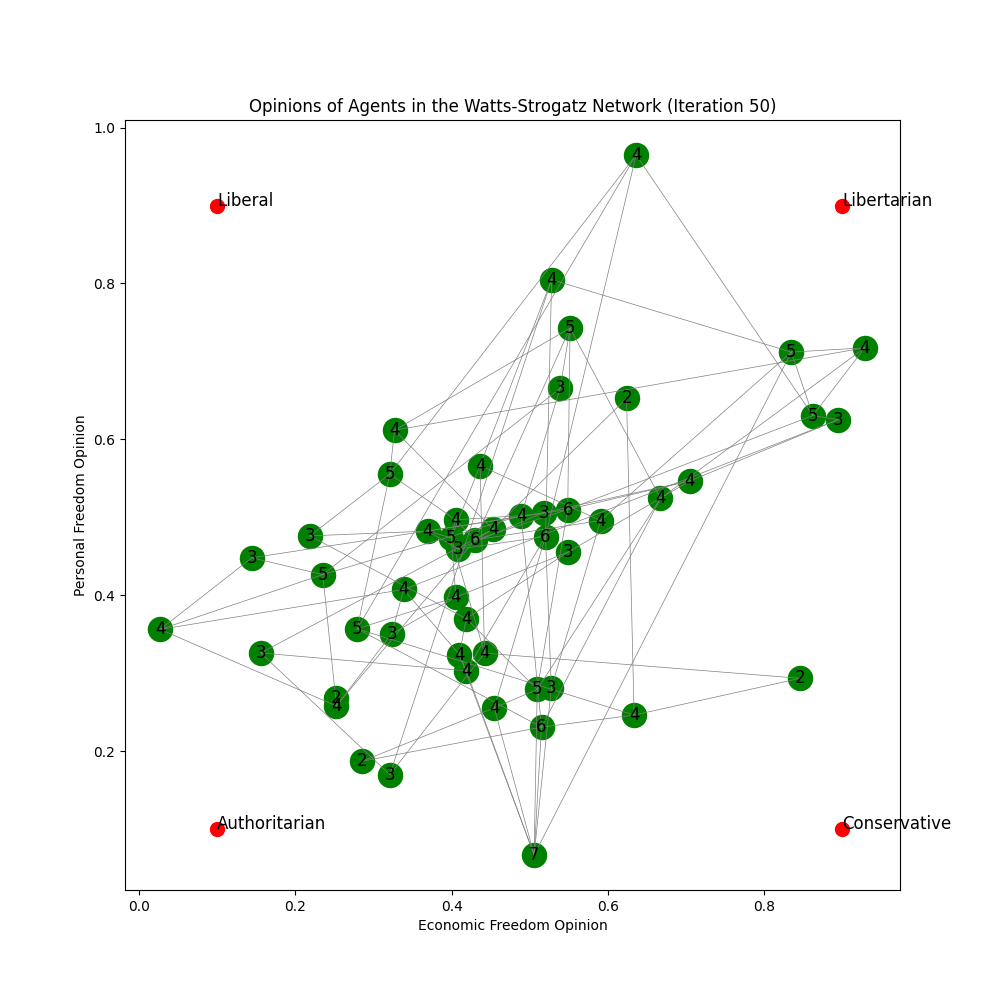
\includegraphics[width=0.5\textwidth]{img/Watts-Strogatz.png}
  \caption{Watts-Strogatz}
  \label{fig:Watts-Strogatz}
\end{figure}

\begin{figure}
  \centering
  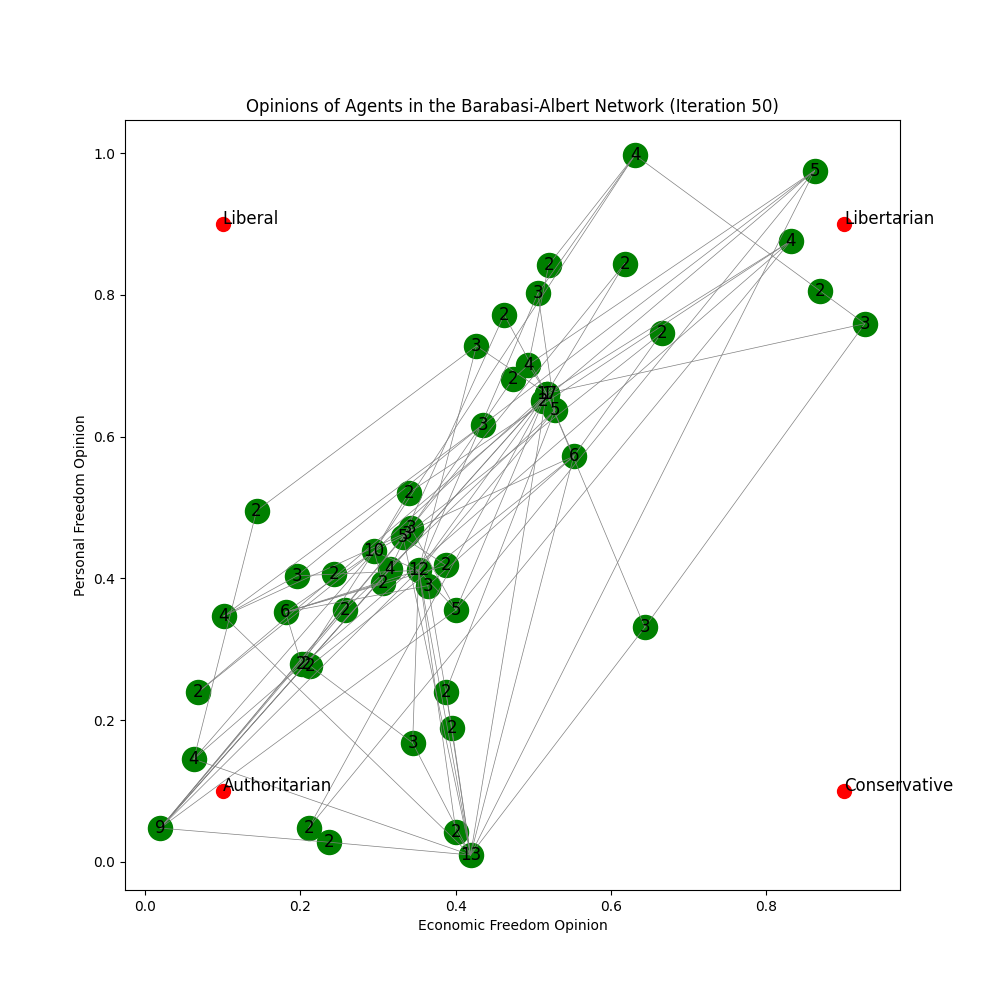
\includegraphics[width=0.5\textwidth]{img/Barabasi-Albert.png}
  \caption{Barabasi-Albert}
  \label{fig:Barabasi-Albert}
\end{figure}

\begin{figure}
  \centering
  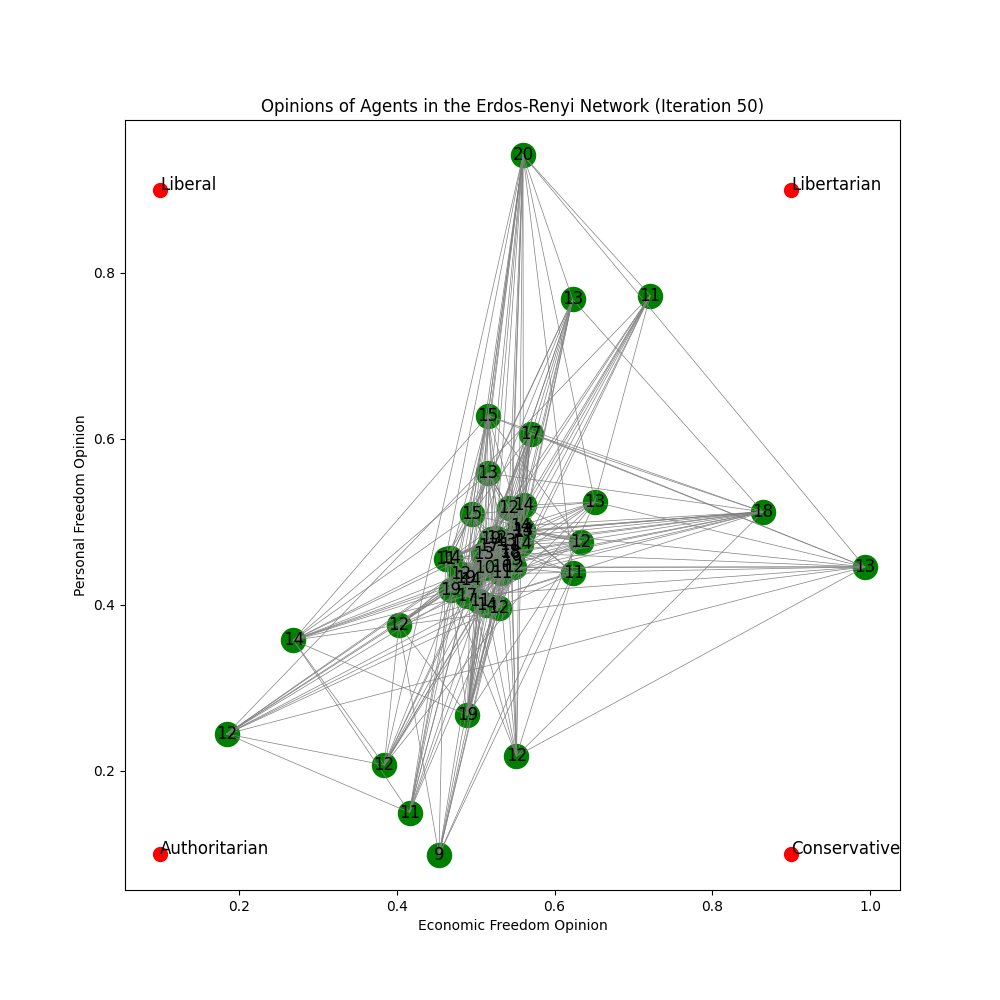
\includegraphics[width=0.5\textwidth]{img/Erdos-Renyi.png}
  \caption{Erdos-Renyi}
  \label{fig:Erdos-Renyi}
\end{figure}


\section{Analiza różnych współczynników modyfikujących średnią rozkładu}

Jako że współczynnik modyfikujący średnią rozkładu pozwolił na uzyskanie lepszych rezultatów niż do tej pory, przeprowadzono badania dla różnych wartości parametru, wyniki są w plikach CSV pod podanym linkiem.

Przeprowadzone zostały obliczenia dla następujących wartości modyfikatora: [0,1, 0,2, 0,5, 1, 2, 5, 10, 20, 50, 100, 200, 500, 1000],
oraz dla następujących wartości populacji: [20, 50, 100, 200, 500, 1000, 2000, 5000].

Niestety, niewiele z nich pozwoliło na uzyskanie więcej niż jednej grupy na wykresie. Wyniki widoczne poniżej.

\begin{figure}
  \centering
  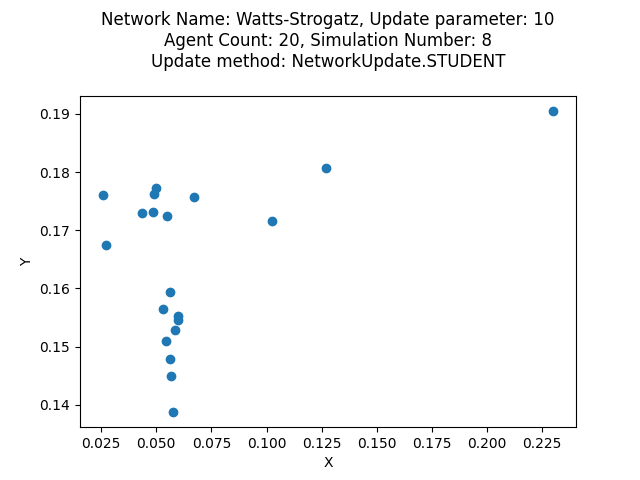
\includegraphics[width=0.5\textwidth]{img/watts_strogatz_10_20_8_student.png}
  \caption{watts strogatz 10 20 8 student}
  \label{fig:watts_strogatz_10_20_8_student}
\end{figure}

\begin{figure}
  \centering
  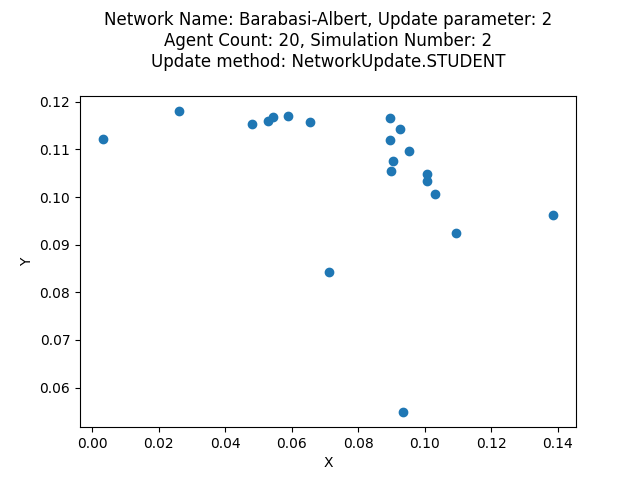
\includegraphics[width=0.5\textwidth]{img/barabasi_albert_2_20_2_student.png}
  \caption{barabasi albert 2 20 2 student}
  \label{fig:barabasi_albert_2_20_2_student}
\end{figure}

\begin{figure}
  \centering
  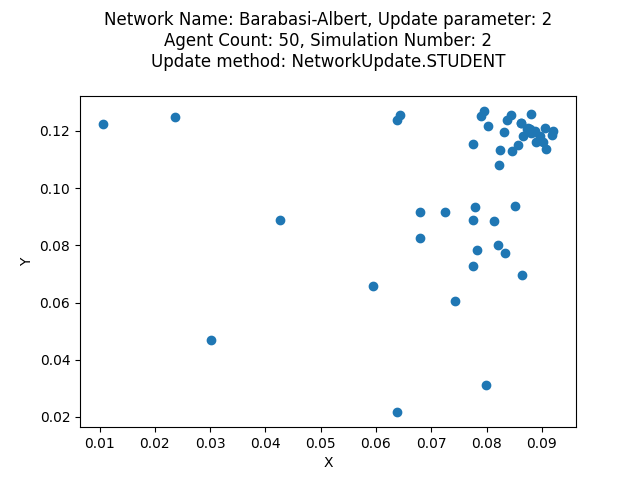
\includegraphics[width=0.5\textwidth]{img/barabasi_albert_2_50_2_student.png}
  \caption{barabasi albert 2 50 2 student}
  \label{fig:barabasi_albert_2_50_2_student}
\end{figure}

\begin{figure}
  \centering
  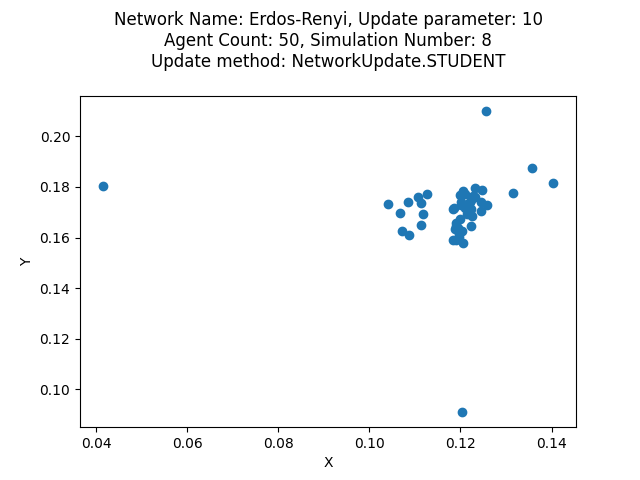
\includegraphics[width=0.5\textwidth]{img/erdos_renyi_10_50_8_student.png}
  \caption{erdos renyi 10 50 8 student}
  \label{fig:erdos_renyi_10_50_8_student}
\end{figure}

\begin{figure}
  \centering
  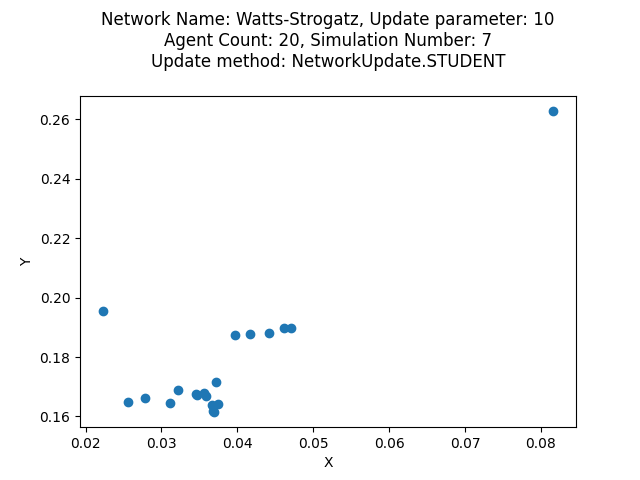
\includegraphics[width=0.5\textwidth]{img/watts_strogatz_10_20_7_student.png}
  \caption{watts strogatz 10 20 7 student}
  \label{fig:watts_strogatz_10_20_7_student}
\end{figure}

%%%%%%%%%%%%%%%%%%%%%%%%%%%%%%%%%%%%%%%%%%%%%%%%%%%%%%%%%%%%%%%%%%%%%%%%%%%%%%%%%%%%%%%%%%%%%%%%%%%%%%%%%%%%%%%%%%%%%%%%%%%%%%%%%%%%%%%%%%%%%%%%%%%%%%%%%%%%%%%%%%%%%%%%%%%%%%%%%%%%%%%%%%%%%%%%%%%%%%%%%%%%%%%%%%

\chapter{Analiza otrzymanych wyników}



%%%%%%%%%%%%%%%%%%%%%%%%%%%%%%%%%%%%%%%%%%%%%%%%%%%%%%%%%%%%%%%%%%%%%%%%%%%%%%%%%%%%%%%%%%%%%%%%%%%%%%%%%%%%%%%%%%%%%%%%%%%%%%%%%%%%%%%%%%%%%%%%%%%%%%%%%%%%%%%%%%%%%%%%%%%%%%%%%%%%%%%%%%%%%%%%%%%%%%%%%%%%%%%%%%

\chapter{Podsumowanie}

\listoftables
\listoffigures

\thebibliography{99}
%Rozdział 2.
\bibitem{Tesfatsion2006} Tesfatsion, L., \& Judd, K. L. (Eds.). (2006). \textit{Handbook of Computational Economics: Agent-Based Computational Economics} (Vol. 2). Elsevier.
\bibitem{Epstein2007} Epstein, J. M. (2007). \textit{Generative Social Science: Studies in Agent-Based Computational Modeling}. Princeton University Press.
\bibitem{Grimm2005} Grimm, V., \& Railsback, S. F. (2005). \textit{Individual-based Modeling and Ecology}. Princeton University Press.
\bibitem{Bonabeau2002} Bonabeau, E. (2002). Agent-based modeling: Methods and techniques for simulating human systems. \textit{Proceedings of the National Academy of Sciences}, 99 (Suppl 3), 7280-7287.
\bibitem{Eubank2004} Eubank, S., Guclu, H., Kumar, V. S. A., Marathe, M. V., Srinivasan, A., Toroczkai, Z., \& Wang, N. (2004). Modelling disease outbreaks in realistic urban social networks. \textit{Nature}, 429 (6988), 180-184.

\bibitem{Wasserman1994} Wasserman, S., \& Faust, K. (1994). \textit{Social Network Analysis: Methods and Applications}. Cambridge University Press.
\bibitem{Newman2010} Newman, M. E. J. (2010). \textit{Networks: An Introduction}. Oxford University Press.
\bibitem{Girvan2002} Girvan, M., \& Newman, M. E. J. (2002). Community structure in social and biological networks. \textit{Proceedings of the National Academy of Sciences}, 99 (12), 7821-7826.
\bibitem{Freeman1979} Freeman, L. C. (1979). Centrality in social networks: Conceptual clarification. \textit{Social Networks}, 1(3), 215-239.
\bibitem{Hanneman2005} Hanneman, R. A., \& Riddle, M. (2005). \textit{Introduction to Social Network Methods}. University of California.
\bibitem{Scott2000} Scott, J. (2000). \textit{Social Network Analysis: A Handbook} (2nd ed.). SAGE Publications.
\bibitem{Borgatti1997} Borgatti, S. P., \& Everett, M. G. (1997). Network analysis of two-mode data. \textit{Social Networks}, 19(3), 243-269.
\bibitem{Holme2012} Holme, P., \& Saramäki, J. (2012). Temporal networks. \textit{Physics Reports}, 519(3), 97-125.

\bibitem{Erdos1959} Erdős, P., \& Rényi, A. (1959). On Random Graphs I. \textit{Publicationes Mathematicae}, 6, 290-297.

\bibitem{Barabasi1999} Barabási, A.-L., \& Albert, R. (1999). Emergence of Scaling in Random Networks. \textit{Science}, 286 (5439), 509-512.

\bibitem{Watts1998} Watts, D. J., \& Strogatz, S. H. (1998). Collective dynamics of 'small-world' networks. \textit{Nature}, 393 (6684), 440-442.

\bibitem{Nolan1971} Nolan, D. (1971). The Case for a Libertarian Political Party. \textit{The Individualist}, 1(4), 3-6.

% Rozdział 4.
\bibitem{NetworkX} Hagberg, A. A., Schult, D. A., \& Swart, P. J. (2008). Exploring network structure, dynamics, and function using NetworkX. In \textit{Proceedings of the 7th Python in Science Conference (SciPy2008)} (pp. 11-15). \url{https://networkx.org/}
\bibitem{Matplotlib} Hunter, J. D. (2007). Matplotlib: A 2D graphics environment. \textit{Computing in Science \& Engineering}, 9(3), 90-95. \url{https://matplotlib.org/}
\bibitem{CSV} Python Software Foundation. (n.d.). \textit{csv – CSV File Reading and Writing}. Python Documentation. \url{https://docs.python.org/3/library/csv.html}

% Rozdział 6.
\bibitem{rozklad_trojkatny_wykres} CC BY-SA 3.0, https://commons.wikimedia.org/w/index.php?curid=182090
\bibitem{rozklad_wykladniczy_wykres} Autorstwa Cburnett - Praca własna, CC BY-SA 3.0, https://commons.wikimedia.org/w/index.php?curid=73793

\end{document}
